\section{Question 3}
\begin{equation}
	G(s) = \dfrac{K\exp(-\tau s)}{s(s^2 + s + a)}, \quad \tau>0, \quad a > 0, \quad K > 0
\end{equation}
The transfer function in which s is replaced by $j\omega$ where $\omega$ is frequency.

% The phase angle:
% $$
% \angle G(jw) = \left. \angle K \right. - (\angle j\omega + \left.\angle \left((j\omega)^2 + j\omega + a \right))\right.
% $$
% $$
% \angle G(jw) = \left. \angle K \right. - (\angle j\omega + \left.\angle \left(j\omega -\omega^2 + a \right))\right.
% $$
% $$
% \angle G(jw) = \tan^{-1}\left(\dfrac{0}{K}\right) - \tan^{-1}\left(\dfrac{\omega}{0}\right) - \tan^{-1}\left(\dfrac{\omega}{a - \omega^2}\right)
% $$
% $$
% \angle G(jw) = 0^{\circ} - 90^{\circ} - \tan^{-1}\left(\dfrac{\omega}{a - \omega^2}\right) = 0 - \dfrac{\pi}{2} - \tan^{-1}\left(\dfrac{\omega}{a - \omega^2}\right)
% $$
% The amplitude ratio:
% $$
% \left\vert G(j\omega) \right\vert = \left\vert \dfrac{K}{j\omega\left((j\omega)^2 + j\omega + a \right)} \right\vert 
% =  \left\vert \dfrac{K}{j\omega\left(j\omega -\omega^2 + a\right)} \right\vert
% $$
% $$
% \left\vert G(j\omega) \right\vert = \dfrac{\left\vert K \right\vert}{\left\vert j\omega \right\vert
% \left\vert j\omega -\omega^2 + a \right\vert
% } = \dfrac{K}{\omega\sqrt{\omega^2 + (\omega^2-a)^2}}
% $$
Cause $a>0$ we have just on pole on imaginary axis.
\begin{figure}[H]
	\caption{Contour near the origin of the s plane and closed contour in the s plane}
	\centering
	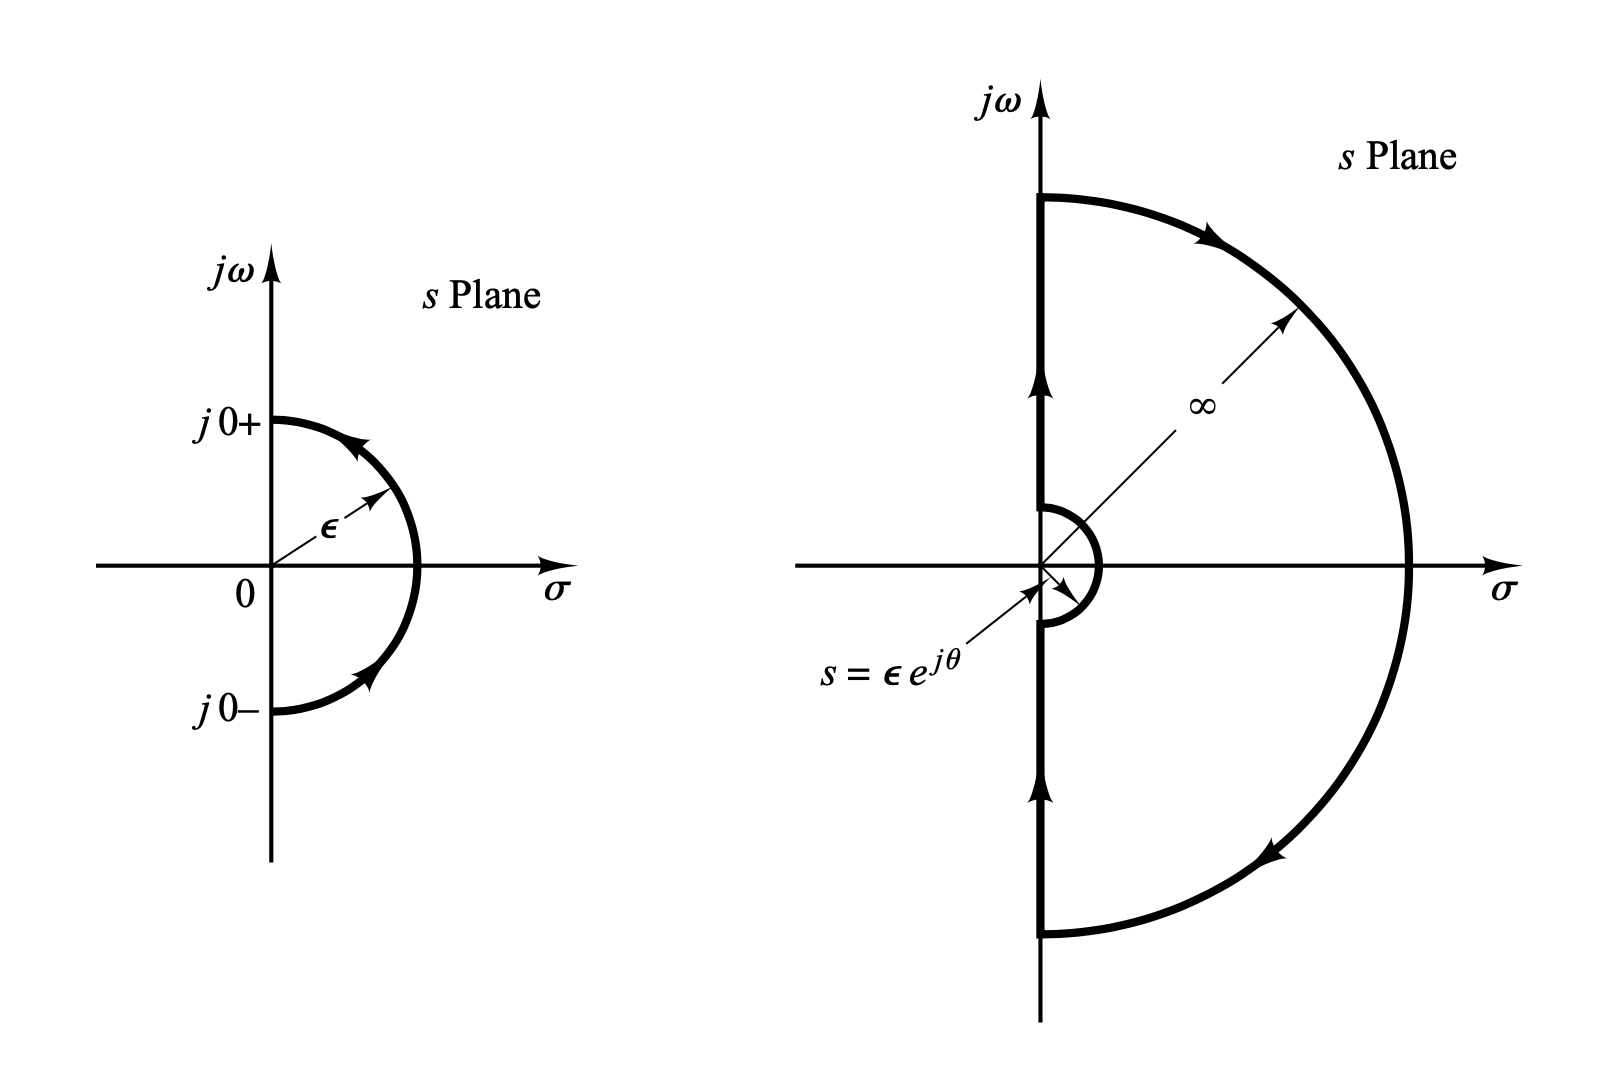
\includegraphics[width=12cm]{../Figure/Q2/nyquist_s_plane.png}
\end{figure}
On the semicircular path with radius $\epsilon$ (where $\epsilon \ll 1 $), the complex variable s can be written
$$
s = \epsilon \exp(j\theta)
$$
where $\theta$ varies from $-\dfrac{\pi}{2}$ to $\dfrac{\pi}{2}$.
\begin{figure}[H]
	\caption{s-Plane}
	\centering
	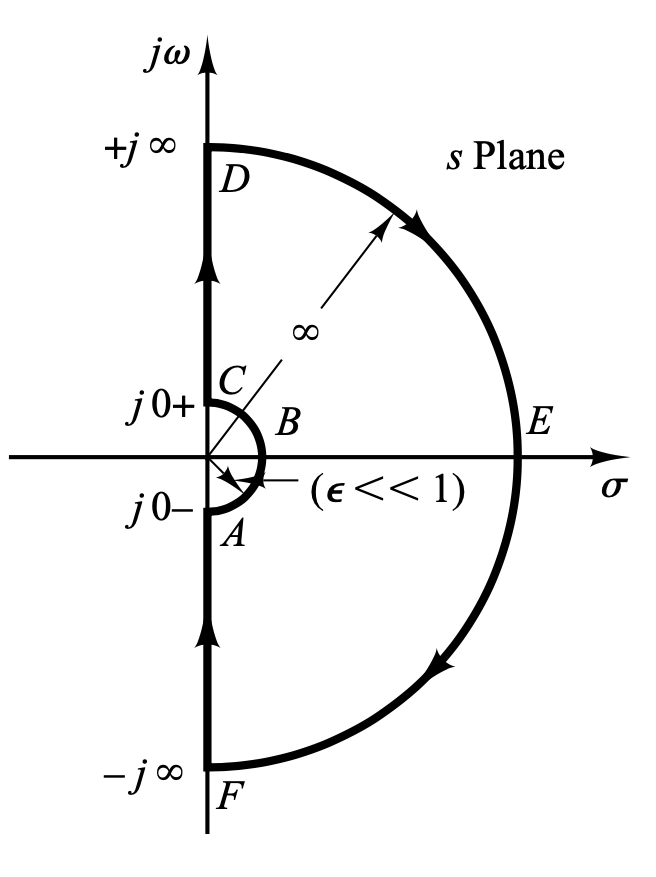
\includegraphics[width=12cm]{../Figure/Q2/nyquist_s_plane_name.png}
\end{figure}
Now we calculate $j\omega$ in A, C, D and F.

A:

$s = j\omega,\quad \omega = -\epsilon$
$$
 \lim_{\omega\to -\epsilon}G(j\epsilon)  = \dfrac{K\exp(\tau j\epsilon)}{-j\epsilon((j\epsilon)^2 - j\epsilon + a)} = \dfrac{K\exp(\tau j\omega)}{-j\epsilon(-\epsilon^2 - j\epsilon + a)} = \dfrac{K\exp(\tau j\epsilon)}{j\epsilon^3 - \epsilon^2 - aj\epsilon}
$$
$$
\lim_{\epsilon \to 0}\dfrac{K\exp(\tau j\epsilon)}{j\epsilon^3 - \epsilon^2 - aj\epsilon} = \lim_{\epsilon \to 0} \dfrac{K\exp(\tau j\epsilon)}{-aj\epsilon} = \lim_{\epsilon \to 0} \dfrac{Kj\exp(\tau j\epsilon)}{a\epsilon} =  \infty \angle 90^{\circ}
$$

C:

$s = j\omega,\quad \omega = \epsilon$
$$
 \lim_{\omega\to \epsilon}G(j\omega)  = \dfrac{K\exp(-\tau j\epsilon)}{j\epsilon((j\epsilon)^2 + j\epsilon + a)} = \dfrac{K\exp(-\tau j\epsilon)}{j\epsilon(-\epsilon^2 + j\epsilon + a)} = \dfrac{K\exp(-\tau j\epsilon)}{j\epsilon^3 - \epsilon^2 - aj\epsilon}
$$
$$
\lim_{\epsilon \to 0}\dfrac{K\exp(-\tau j\epsilon)}{j\epsilon^3 - \epsilon^2 + aj\epsilon} = \lim_{\epsilon \to 0} \dfrac{K\exp(-\tau j\epsilon)}{-aj\epsilon} = \lim_{\epsilon \to 0} \dfrac{-Kj\exp(-\tau j\epsilon)}{a\epsilon} =  \infty \angle -90^{\circ}
$$

A to C:

$s = j\omega,\quad \omega = \epsilon\exp(j\theta), \quad \theta: -\dfrac{\pi}{2}\to 0 \to \dfrac{\pi}{2}(CCW)$
$$
 \lim_{\epsilon\to 0}G(\epsilon\exp(j\theta))  =\dfrac{K\exp(-\tau j\epsilon)}{\epsilon\exp(j\theta)((\epsilon\exp(j\theta))^2 + \epsilon\exp(j\theta) + a)} =  \dfrac{K\exp(-\tau j\epsilon)}{\epsilon^3\exp(3j\theta) + \epsilon^2\exp(2j\theta) + a\epsilon\exp(j\theta)} 
$$
$$
\lim_{\epsilon \to 0}\dfrac{K\exp(-\tau j\epsilon)}{a\epsilon\exp(j\theta)} = \lim_{\epsilon \to 0} \dfrac{K\exp(-j\theta-\tau j \epsilon)}{a\epsilon} =  \infty \angle -\theta 
$$

D:

$s = j\omega,\quad \omega = \infty$
$$
\lim_{\omega\to \infty}G(j\omega)  =  \lim_{\omega\to \infty}\dfrac{K\exp(-\tau j\omega)}{j\omega((j\omega)^2 + j\omega + a)} = \lim_{\omega\to \infty} \dfrac{K\exp(-\tau j\omega)}{j\omega(-\omega^2 + j\omega + a)} = \lim_{\omega\to \infty} \dfrac{K\exp(-\tau j\omega)}{-j\omega^3 - \omega^2 + aj\omega}
$$
$$
\lim_{\omega\to \infty} \dfrac{K\exp(-\tau j\omega)}{-j\omega^3} = \lim_{\omega\to \infty} \dfrac{jK\exp(-\tau j\omega)}{\omega^3}  
= 0 \angle 90^{\circ}
$$

F:

$s = j\omega,\quad \omega = -\infty$
$$
\lim_{\omega\to -\infty}G(j\omega)  =  \lim_{\omega\to -\infty}\dfrac{K\exp(-\tau j\omega)}{j\omega((j\omega)^2 + j\omega + a)} = \lim_{\omega\to -\infty} \dfrac{K\exp(-\tau j\omega)}{j\omega(-\omega^2 + j\omega + a)} = \lim_{\omega\to -\infty} \dfrac{K\exp(-\tau j\omega)}{-j\omega^3 - \omega^2 + aj\omega}
$$
$$
\lim_{\omega\to -\infty} \dfrac{K\exp(-\tau j\omega)}{-j\omega^3} = \lim_{\omega\to -\infty} \dfrac{jK\exp(-\tau j\omega)}{\omega^3}  
= 0 \angle -90^{\circ}
$$

\begin{figure}[H]
	\caption{Nyquist plot using MATLAB ($a = 1, K = 1, \tau = 0.01$)}
	\centering
	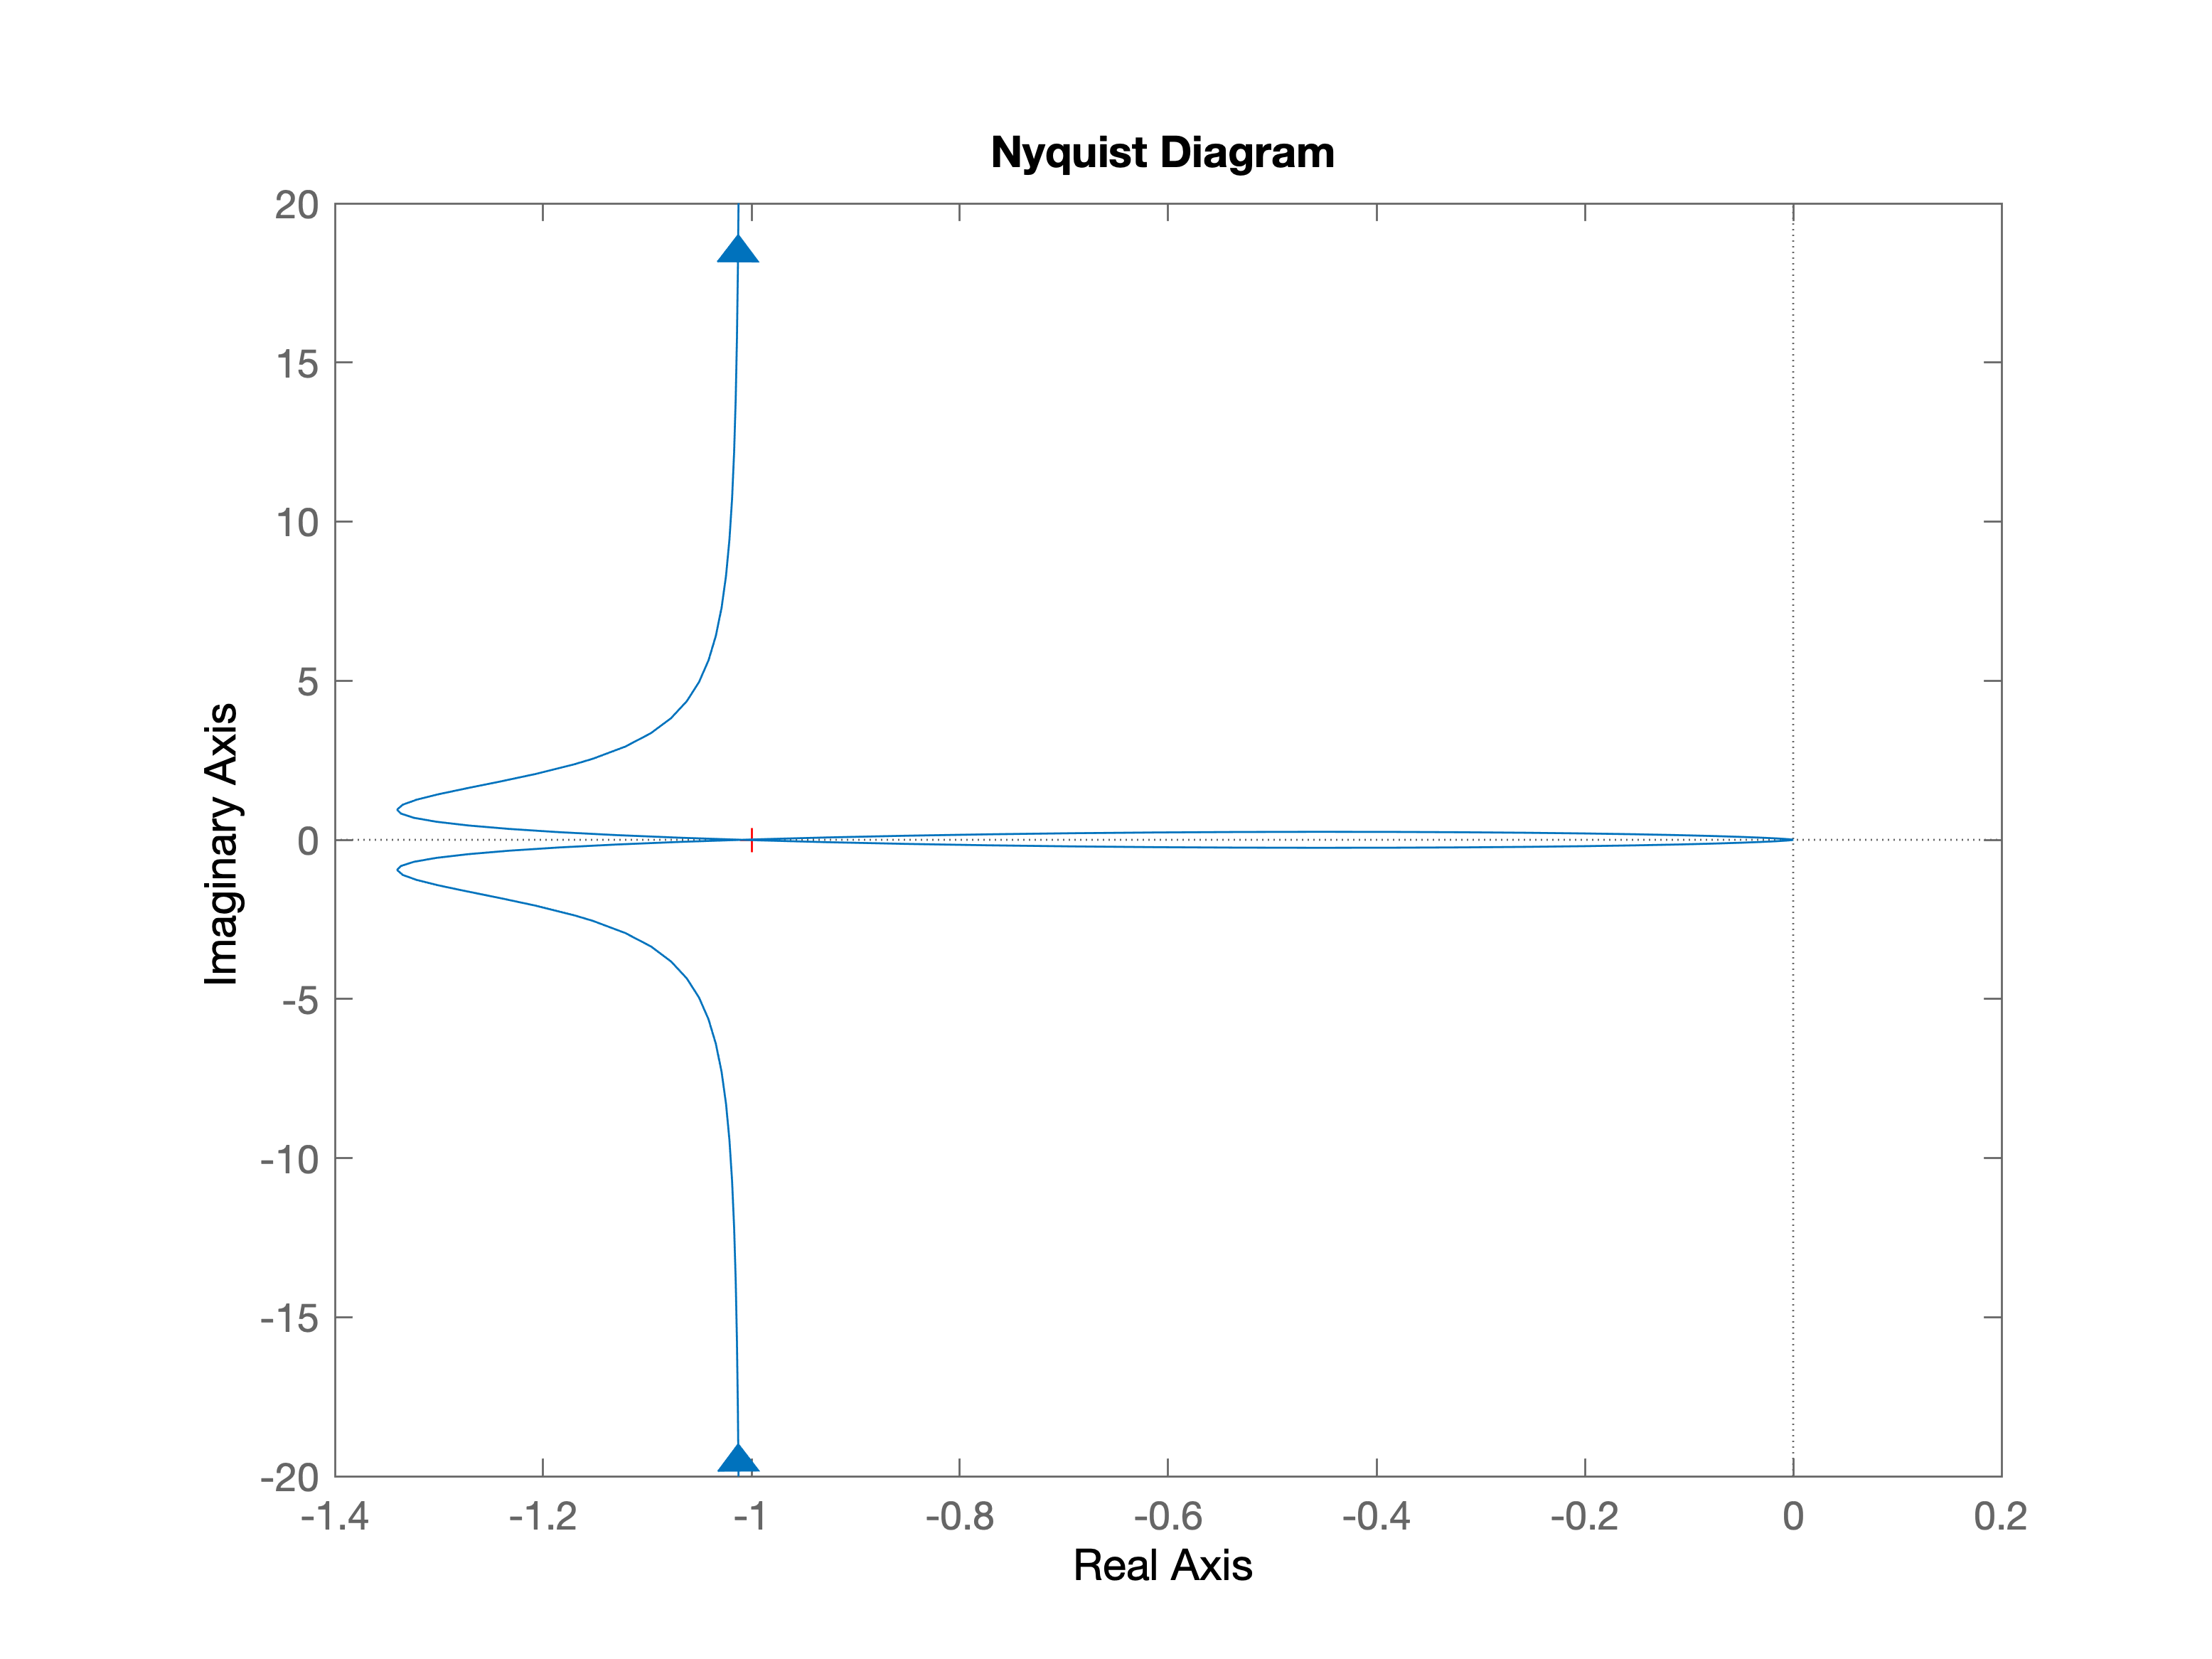
\includegraphics[width=12cm]{../Figure/Q3/MATLAB-Nyquist.png}
\end{figure}

Now we know shape of nyquist plot. we find out where it's equal to $-1$.

$$
G(j\omega) = -1 + 0j = \dfrac{K\exp(-\tau j\omega)}{j\omega((j\omega))^2 + j\omega + a)} = \dfrac{K\exp(-\tau j\omega)}{-j\omega^3 - \omega^2 + aj\omega} = -1
$$

$$
\to j\omega^3 + \omega^2 -aj\omega = K\exp(-\tau j\omega) \to j\omega^3 + \omega^2 -aj\omega - K\exp(-\tau j\omega) = 0
$$
if we assume $\omega\tau \ll 1$ the problem is like previous question.
Two equation and two unknowns.
\begin{align*}
	j\omega^3 &=aj\omega-Kj\omega\tau \to \omega^2 = a-K\tau\\
	\omega^2 &=K \to \omega^2 = K
\end{align*}
When $a = K$ the nyquist plot cross from $-1$ point. When $a-\tau\omega>K$ the nyquist plot is before $-1$ and when $a-\tau\omega<K$ the nyquist plot cross $-1$ and system is unstable.
\begin{figure}[H]
	\caption{Stable Nyquist plot using MATLAB ($a = 2, K = 1, \tau = 0.01$)}
	\centering
	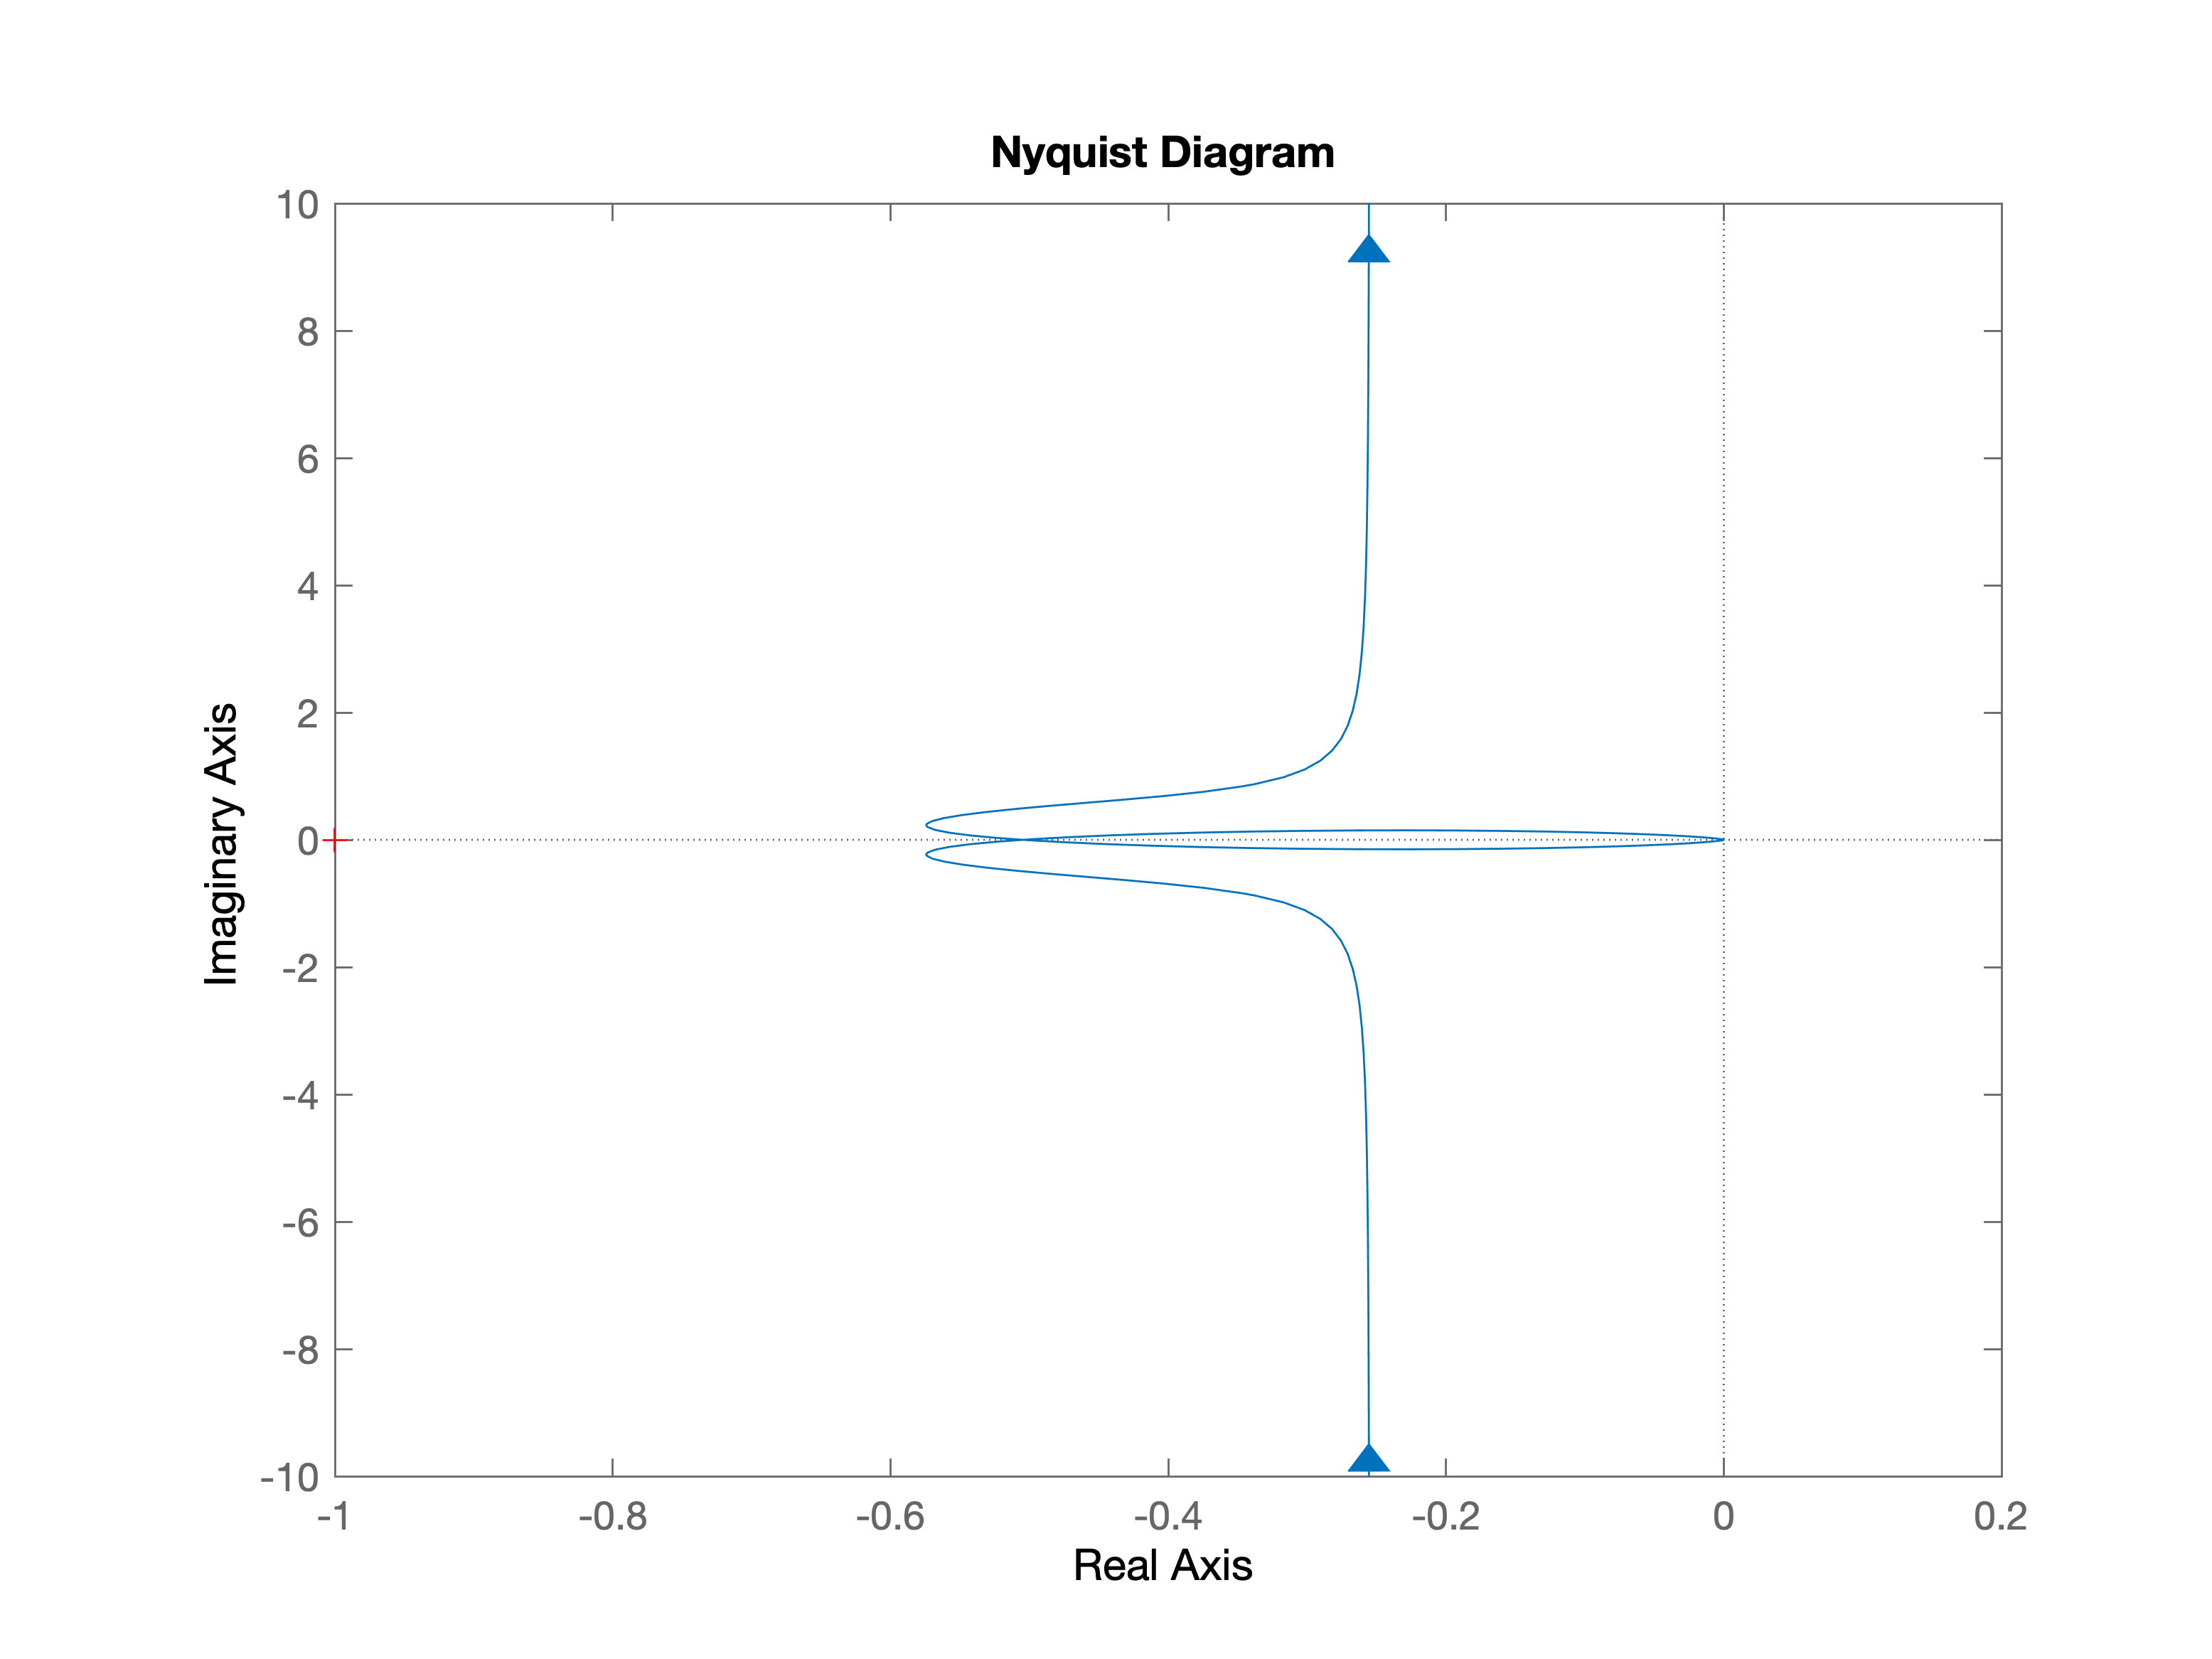
\includegraphics[width=12cm]{../Figure/Q3/MATLAB-Nyquist_stable.png}
\end{figure} 
\begin{figure}[H]
	\caption{Unstable Nyquist plot using MATLAB ($a = 1, K = 2, \tau = 0.01$)}
	\centering
	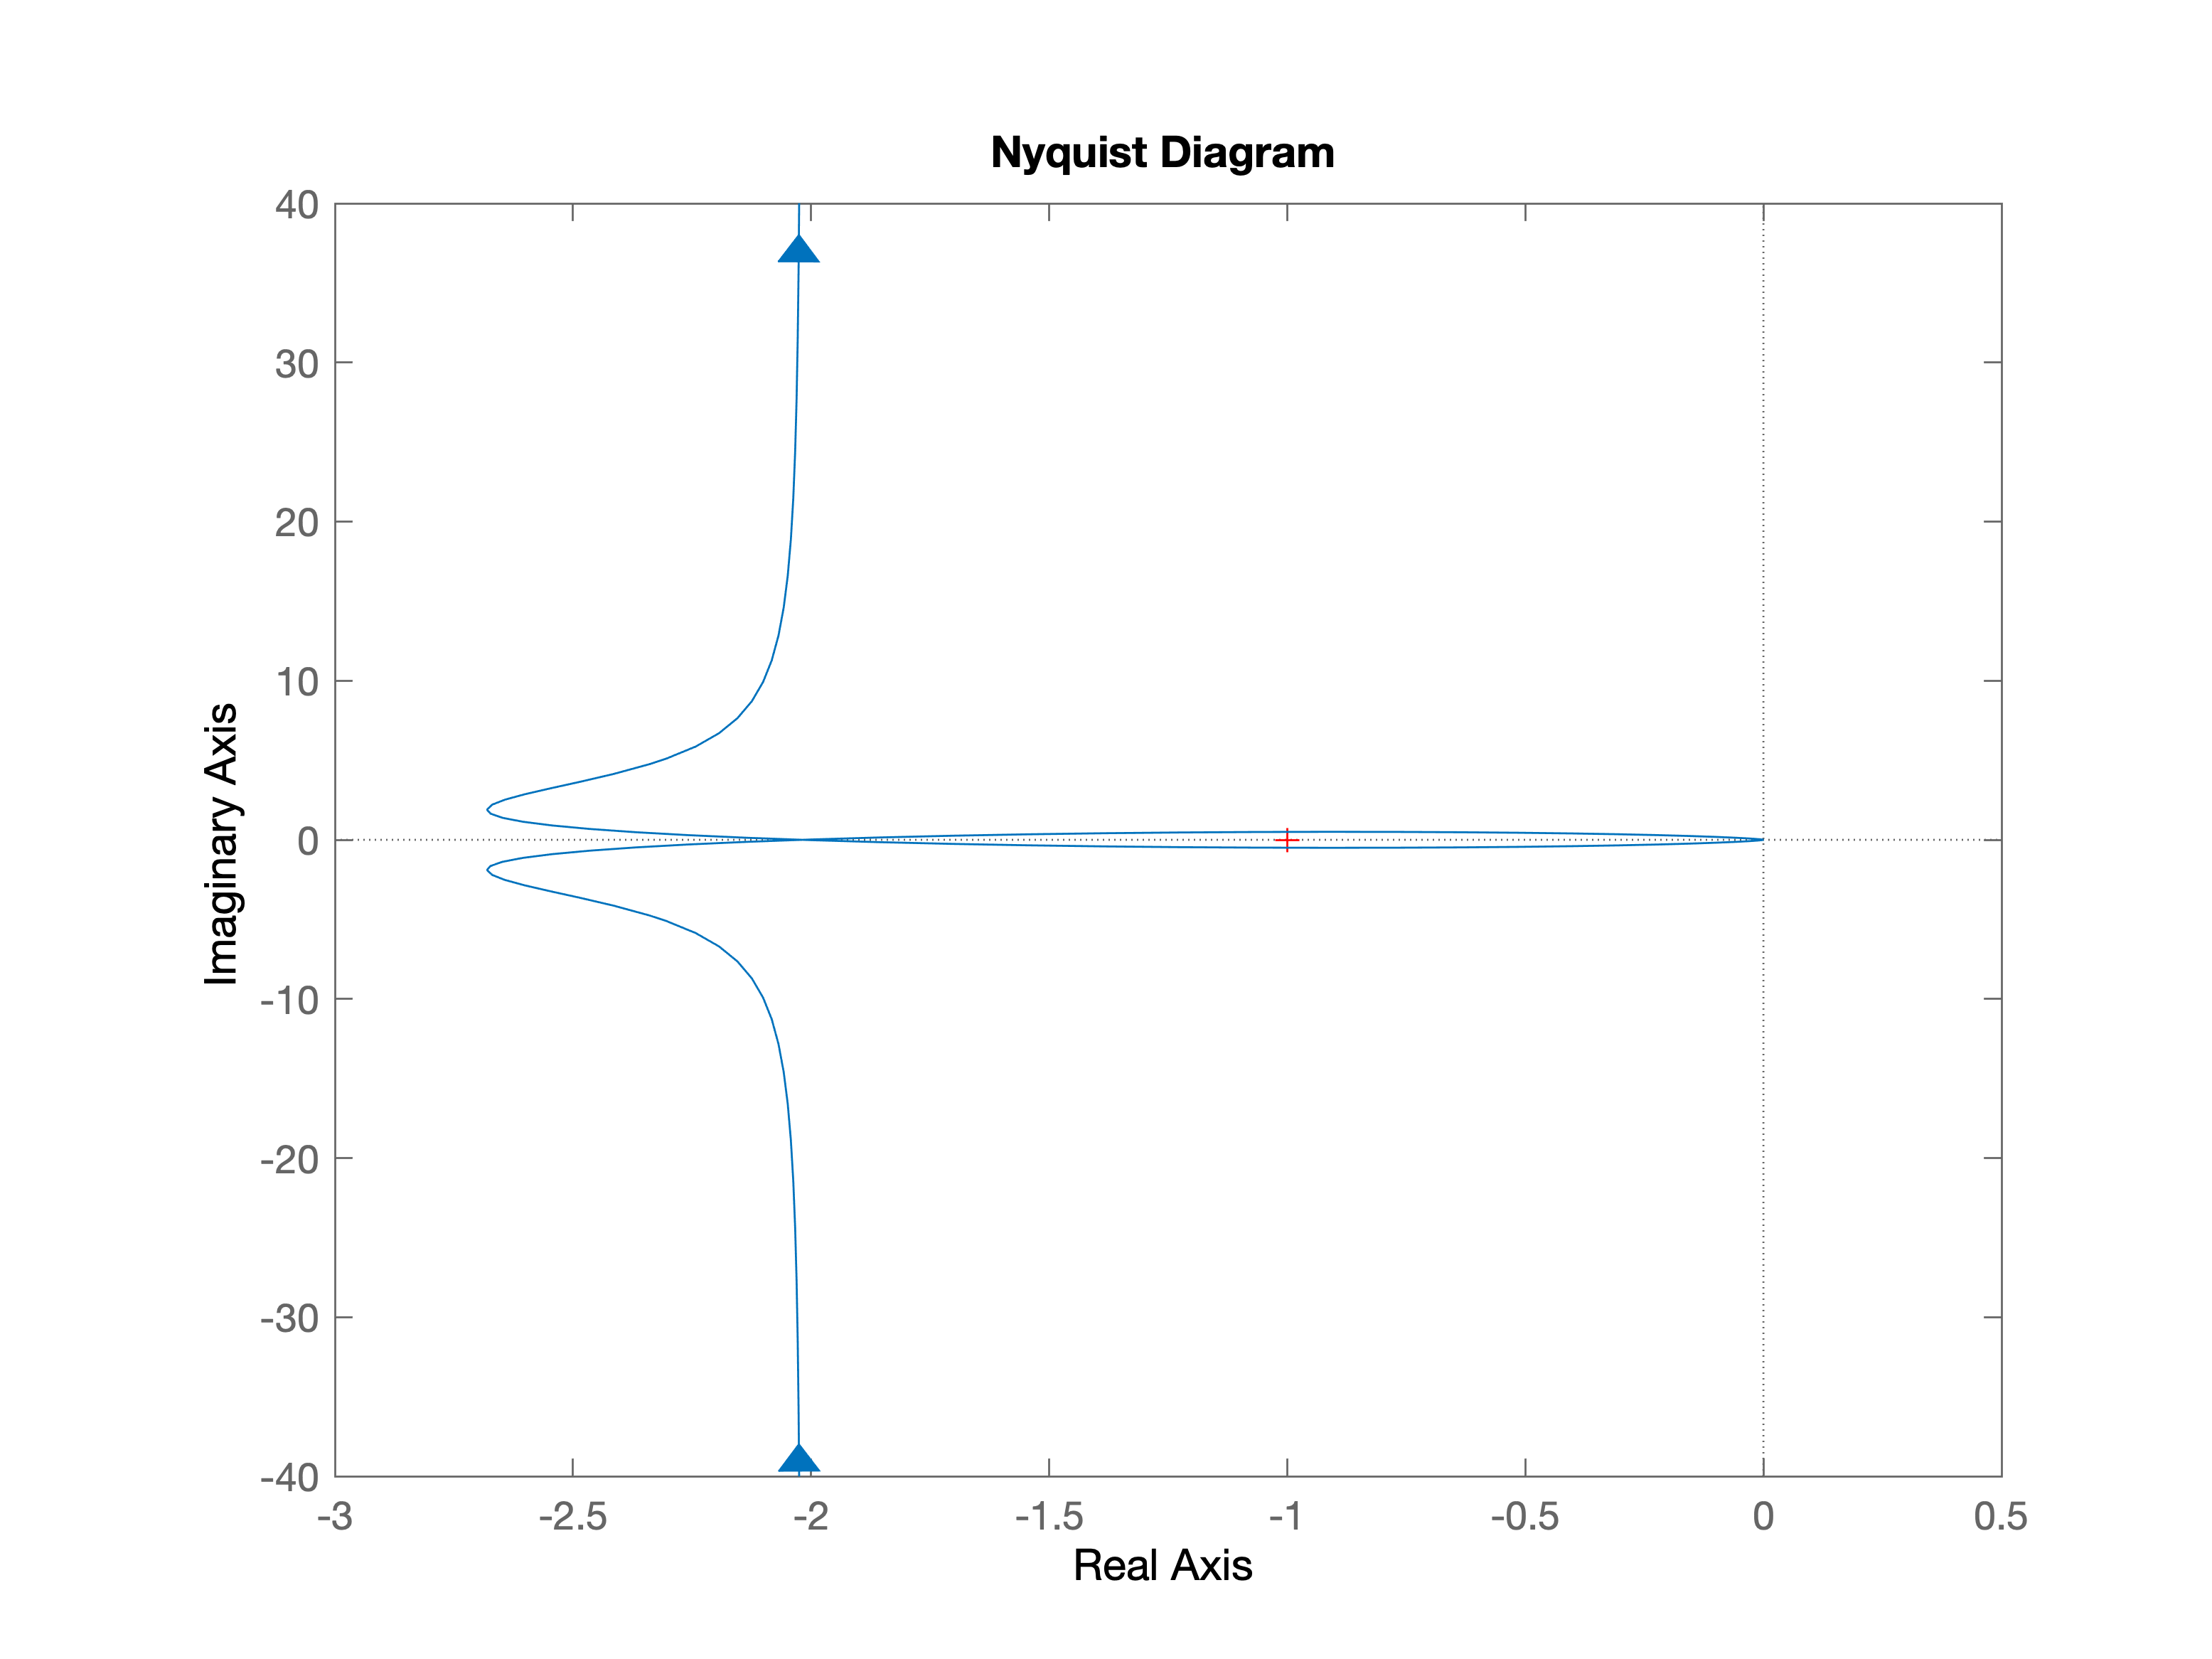
\includegraphics[width=12cm]{../Figure/Q3/MATLAB-Nyquist_unstable.png}
\end{figure}

When $\tau \ll 1$ it's not true and we have nonlinear equation that is hard to slove.
\begin{align*}
	j\omega^3 &=aj\omega - Kj\sin(\tau\omega)\\
	\omega^2 &=K\cos(\tau\omega)
\end{align*}

when $\tau$ increase we must increase $a$ or decrease $K$ for stable system.

\begin{figure}[H]
	\caption{Unstable Nyquist plot using MATLAB ($a = 1, K = 1, \tau = 2$)}
	\centering
	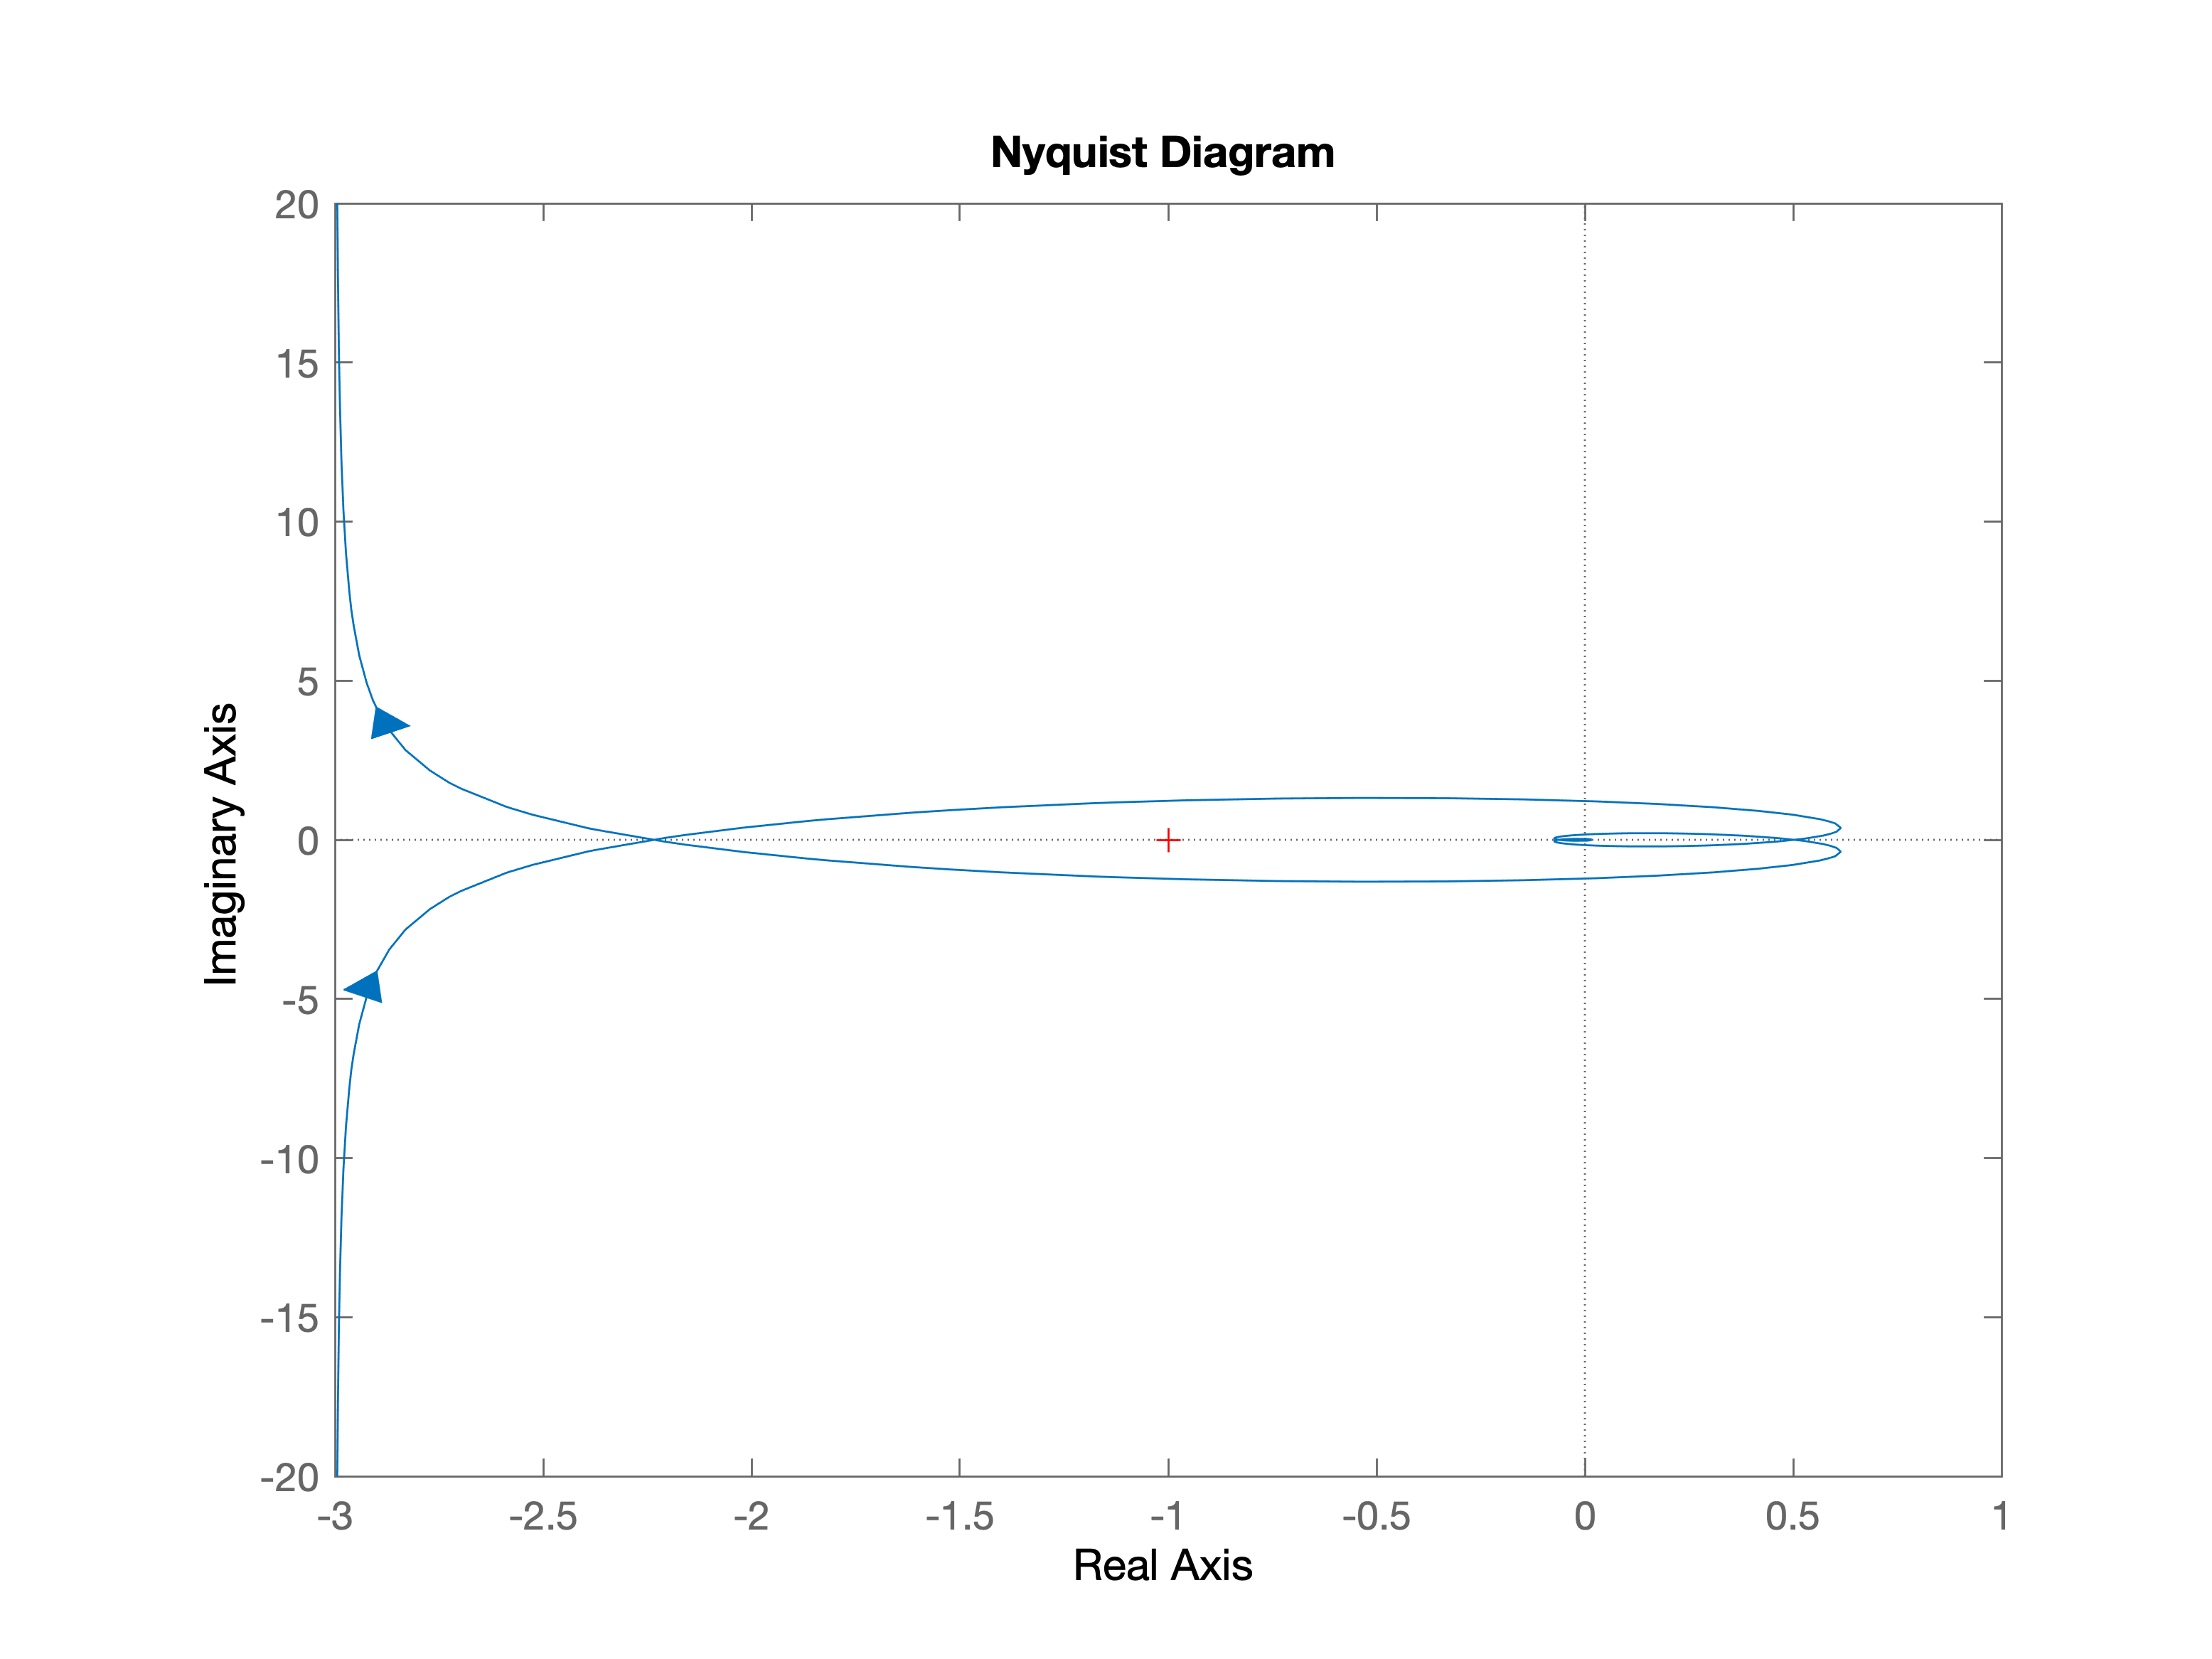
\includegraphics[width=12cm]{../Figure/Q3/MATLAB-Nyquist_increase_tau.png}
\end{figure}

\begin{figure}[H]
	\caption{Stable Nyquist plot using MATLAB ($a = 2, K = 1, \tau = 2$)}
	\centering
	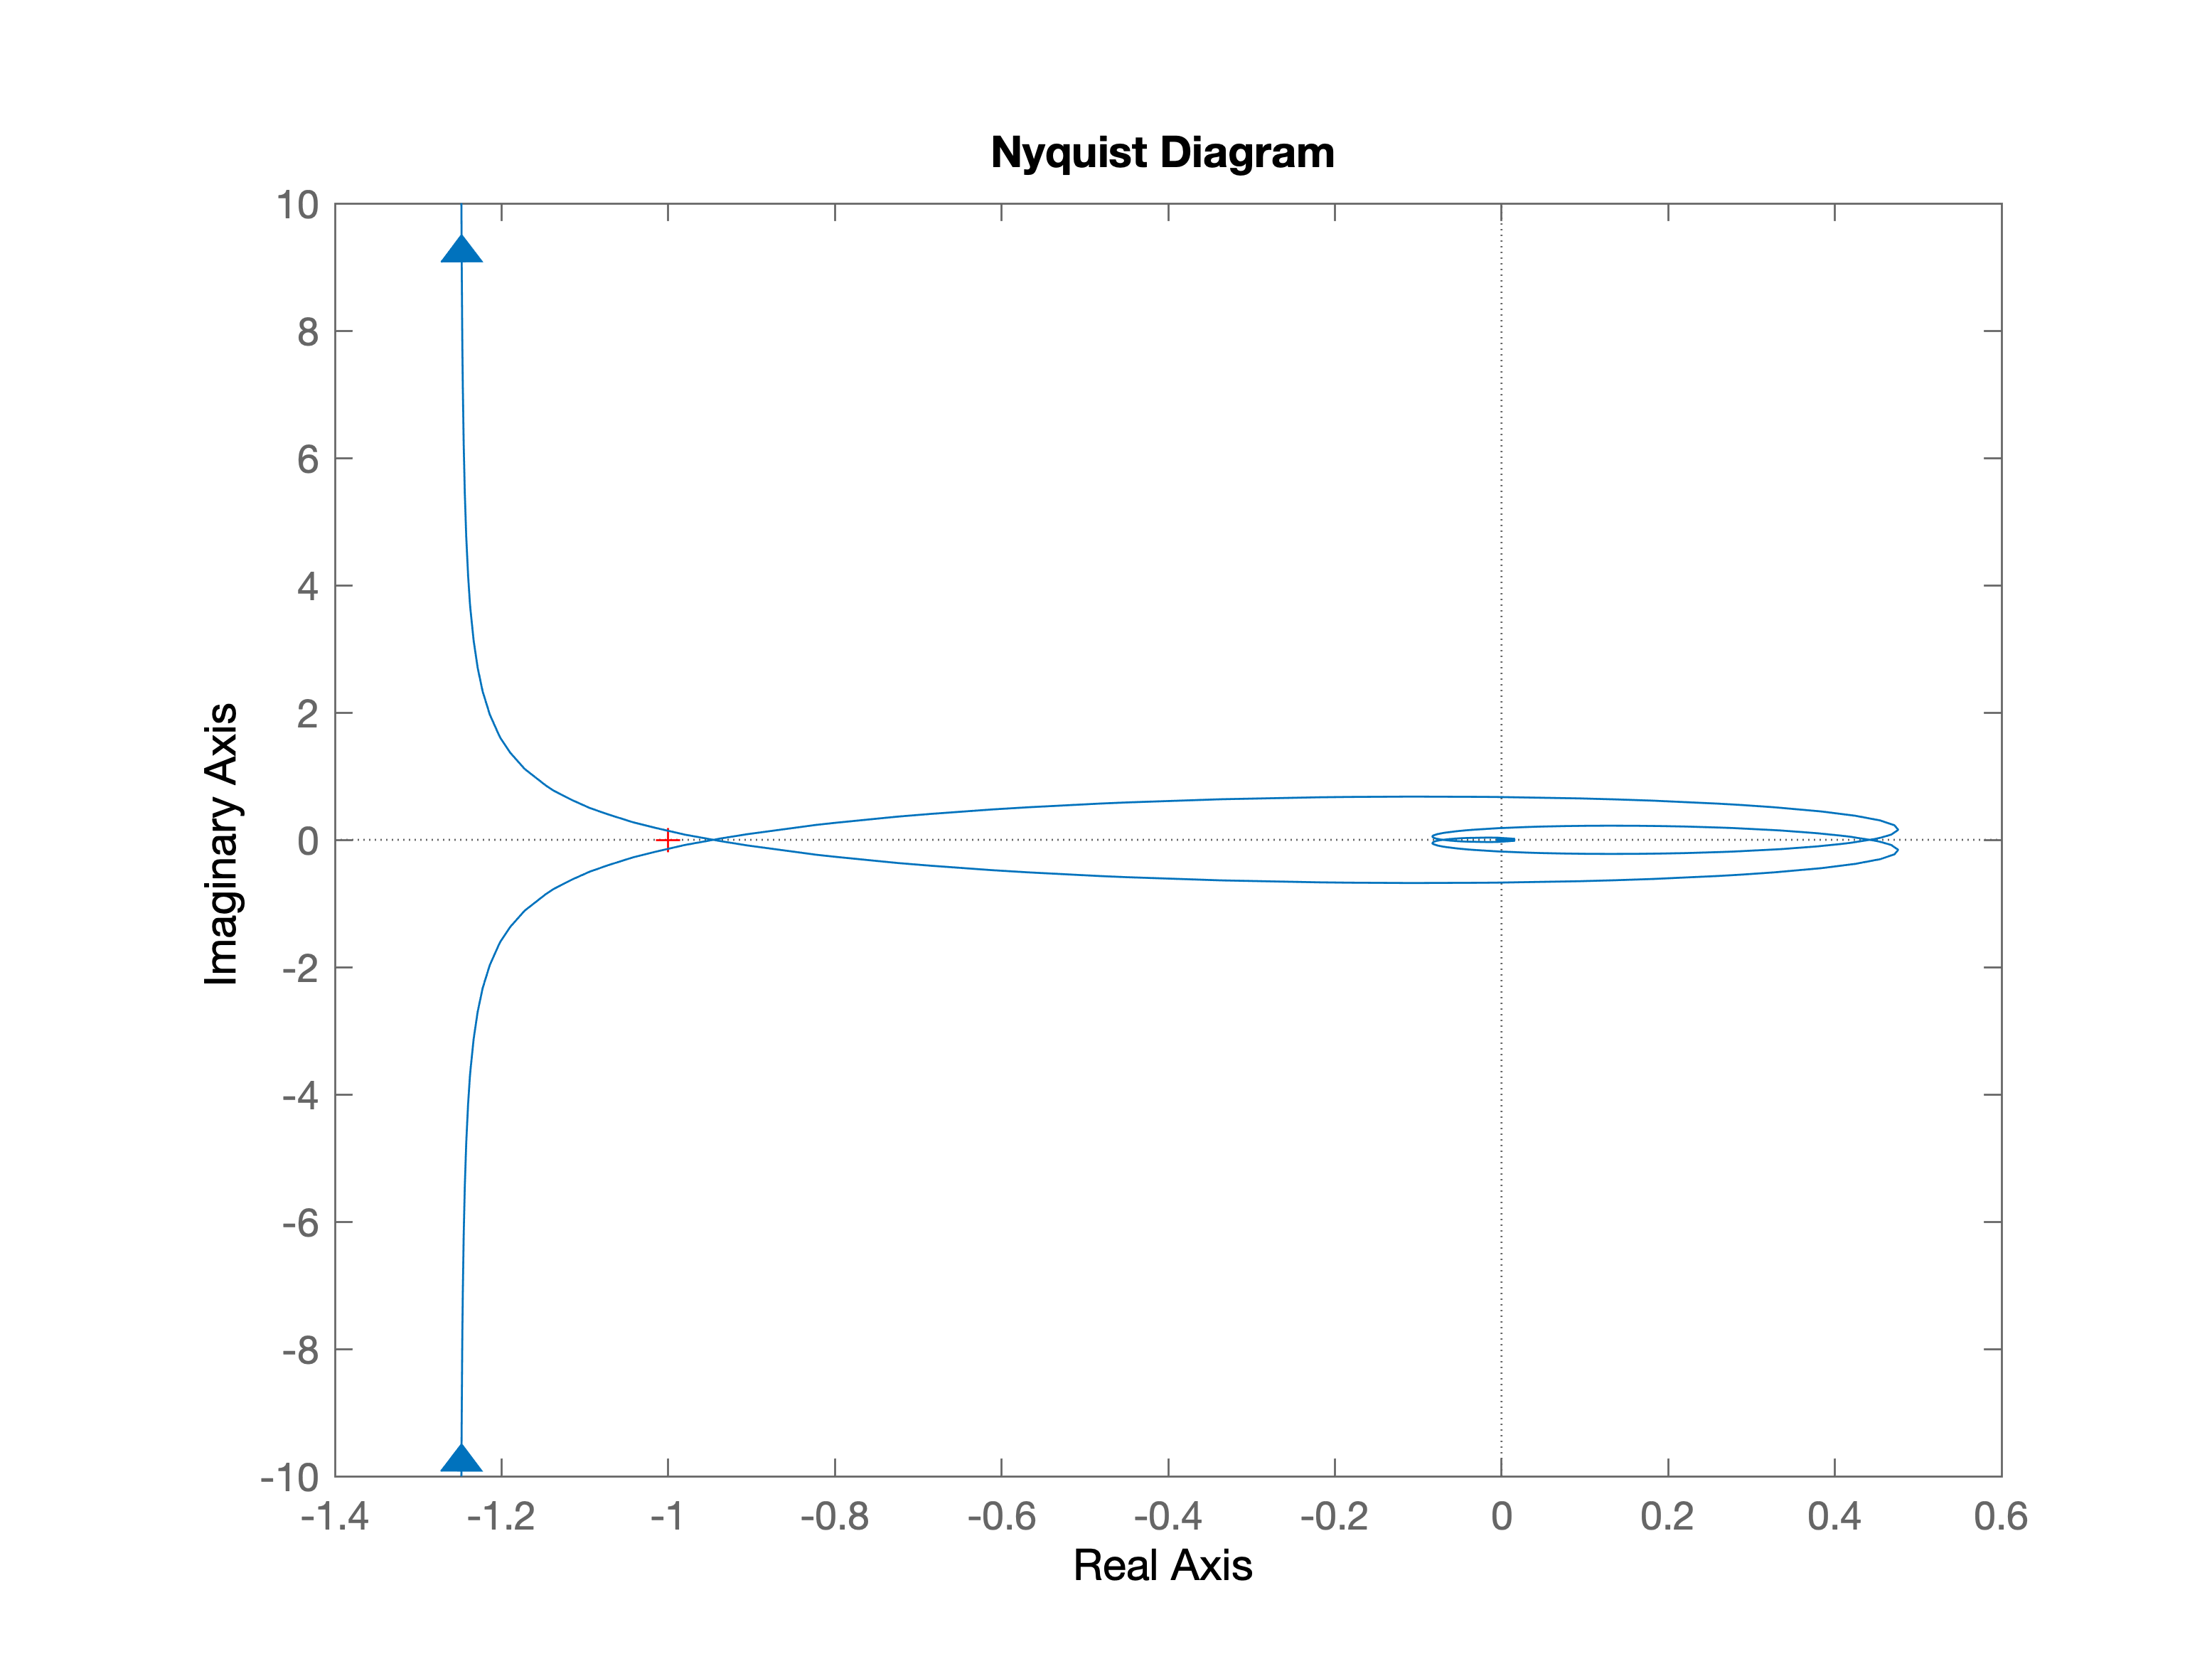
\includegraphics[width=12cm]{../Figure/Q3/MATLAB-Nyquist_increase_tau_and_a.png}
\end{figure}
When we increase $\tau$ it's make our system unstable.

\begin{figure}[H]
	\caption{Unstable Nyquist plot  with large $\tau$ using MATLAB ($a = 2, K = 1, \tau = 100$)}
	\centering
	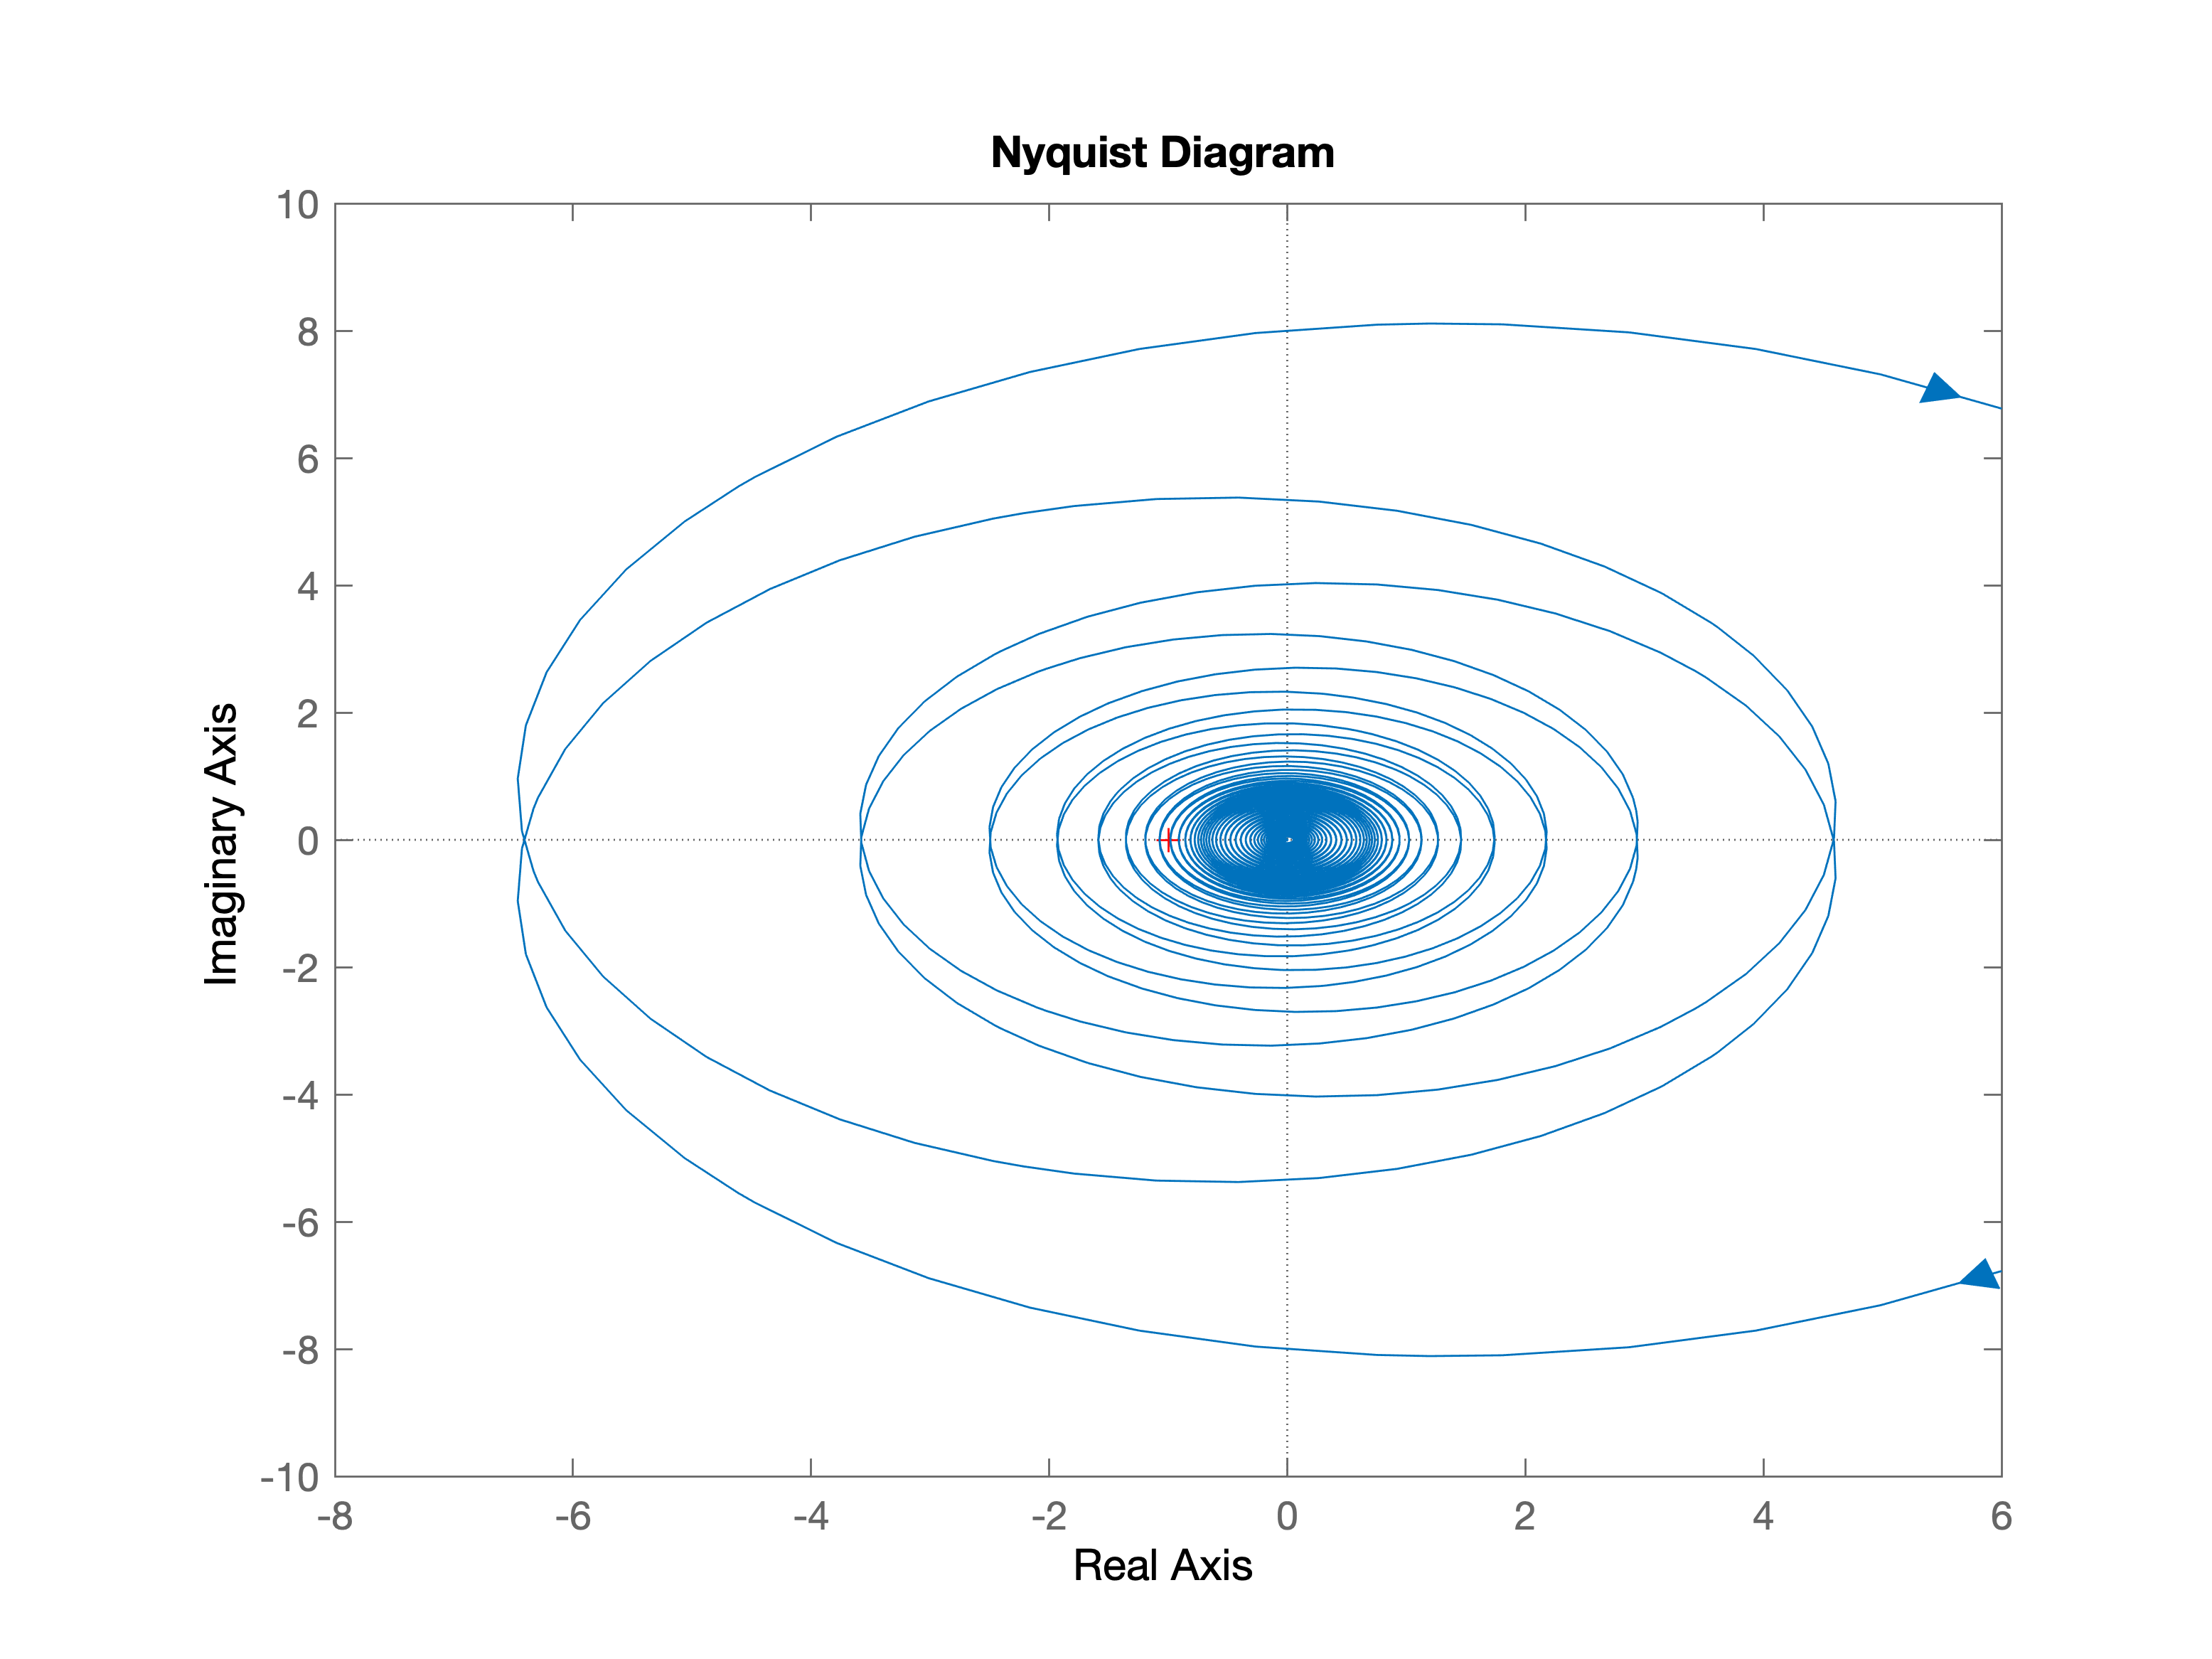
\includegraphics[width=12cm]{../Figure/Q3/MATLAB-Nyquist_increase_tau_very_lage.png}
\end{figure}

\begin{figure}[H]
	\caption{Stable Nyquist plot with large $\tau$ and small $K$ using MATLAB ($a = 2, K = 0.00001, \tau = 100$)}
	\centering
	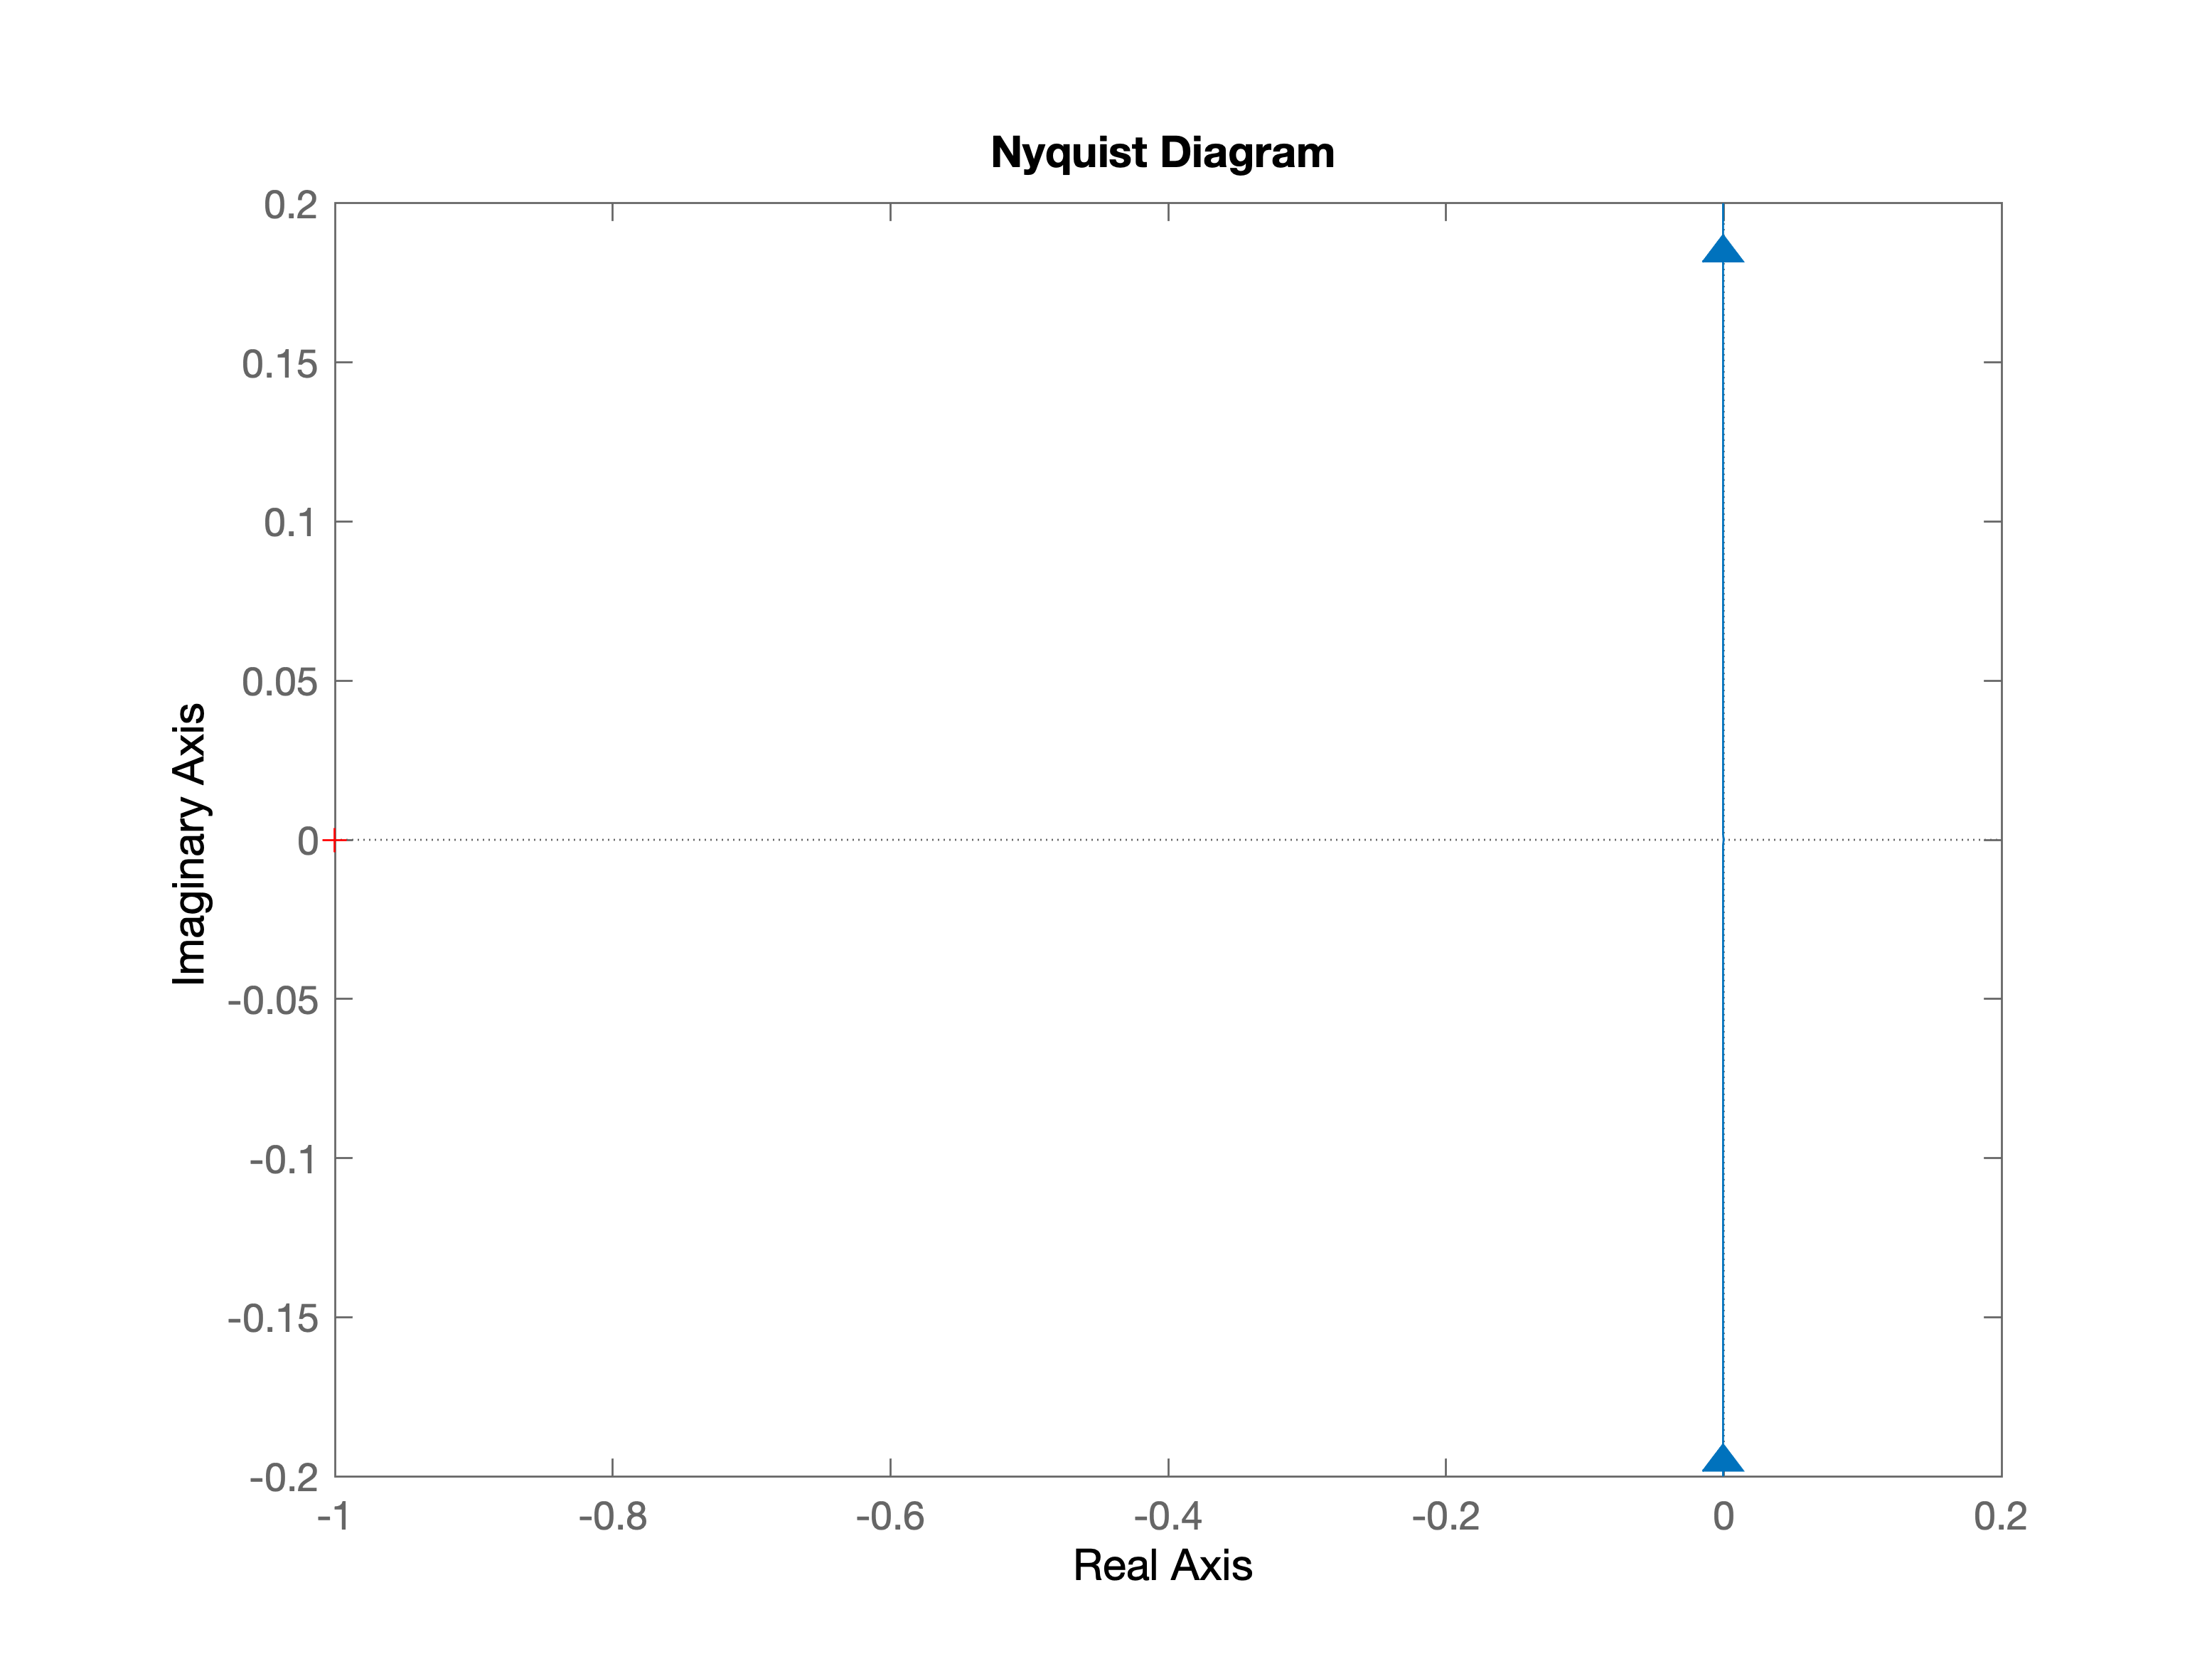
\includegraphics[width=12cm]{../Figure/Q3/MATLAB-Nyquist_increase_tau_very_lage_K_very_low.png}
\end{figure}




